\documentclass[11pt]{article}
\usepackage[english]{babel}

\usepackage[a4paper,margin=3cm,top=2cm]{geometry}
\usepackage[T1]{fontenc}
\usepackage{lmodern}
\usepackage{microtype}
\frenchspacing

\usepackage{natbib}
\bibliographystyle{plainnat}
\usepackage{doi}

\usepackage{graphicx}
\usepackage{xspace}
\usepackage{mathtools}
\usepackage{amssymb}
\usepackage{bm}
\usepackage{xcolor}
\usepackage{enumitem}
\usepackage{booktabs}
\usepackage{pythonhighlight} % for inclusion of Python files
	\lstset{
		style=mypython,basicstyle=\sffamily,frame=lines,
		float,
		numbers=left,numberblanklines=false,
		columns=flexible,keepspaces=true,breaklines}

\newcommand{\nats}{\mathbb{N}}

\DeclareMathOperator*{\argmax}{arg\,max}

\title{Assignment A3: Team XX}
\author{Firstname1 Lastname1 \and Firstname2 Lastname2 \and Firstname3 Lastname3}
\date{}

\begin{document}

\maketitle


\section{Agent Description}\label{sec:description}
Explain, \emph{in your own words}, the workings of your AI agents.
(It can also be a single agent; we use the plural in the rest of this template, but you can replace that by singular if that is your situation.)
Pay special attention to the following:
\begin{itemize}
	\item Include a concise description of the basic agent to which you have added new functionality.
	This is in general your team's A2 agent.
	You are however free to add or even remove functionality that falls in the general ‘minimax’ and ‘heuristic’ categories of the two previous assignments.
	\item Explain all the techniques that you have chosen to implement.
	Consider using pseudocode for this, and then also provide an explanation of the pseudocode.
	(N.B.: The pseudocode does not need to cover all actual code.)
	\item How do your agents use the (unknown) amount of time available for computing the next move? Can they reasonably be expected to find a better move when given more time? Focus on the new features you have included.
	\item Explain the evaluation function used for numerically scoring board positions.
	What is the intuition/reasoning behind it?
	\item For all of the points above, as a general rule of thumb, consider whether the explanation is clear to your fellow students. Whenever you base your design on existing work/methods, provide references to the appropriate literature.
	% You can add comments as well, for example with TODOs.
\end{itemize}
Do not hesitate to go beyond these points above in case relevant aspects of the design are not captured by any of them.

\section{Agent Analysis}\label{sec:analysis}
In contrast to the earlier assignments, you have complete freedom to choose how you analyse (comparative or absolute) agent performance.
The goal is to choose a suite of experiments and analyses that make it possible for you to convincingly discuss the performance of the agents in a wide variety of circumstances (compute-time, board-size, board-type, adversary-type,…).

As before:
\begin{itemize}
	\item Make sure you clearly explain the setup of your experiments.
	\item Create plots and/or tables to summarize the experimental results or provide insight that can be gained from them.
	Basic plots you could use are, for example, those of the average performance (e.g. win/loss/draw statistics) of your agent as a function of compute-time.
\end{itemize}

In your report, include the interesting plots and tables that you have generated.
Also provide some analysis; can you qualitatively summarize the observed performance of your agents on each of these tasks?
Moreover, can you think of a possible explanation for these observations?

\section{Motivation \& Reflection}\label{sec:reflect}
What do you think are strong points of your agents' design and of your experimental design?
Which properties of the problem domain do the agents exploit and which aspects do your experiments test?
Is there an inherent strength to the functionalities you chose for playing the game of competitive sudoku?

Conversely, what do you think are weak points of your agents' design and of your experimental design?
Are there certain properties of the problem domain for which you think your designs are unsuitable?
Which game aspects do your experiments not test?
Is there an inherent weakness to the functionalities you chose for playing the game of competitive sudoku?


\section*{General Guidelines for Your Report}
\textbf{Please remove this section from your submitted report}

This section contains some general guidelines that you should keep in mind when preparing your report:
\begin{itemize}
	\item
		The \textbf{maximum} length of your report is \textbf{7} pages, \textbf{excluding} references and the appendix with your included Python code, but \textbf{including} all figures and tables.
	\item
		Please do not modify the style of the template to squeeze in more content. Make sure all text is legible (not too small).
	\item
		Please carefully proofread your report for typos and grammatical errors; use a spellchecker.
	\item
		References to literature are best added in the \texttt{report\_template.bib} BibTeX file, and invoked in your report using a citation command. For example, “\citet{shannon1950xxii} proposed an approach for \dots” or “\dots as discussed in the literature \citep{shannon1950xxii}”.
	\item
		Tables can be added through the \texttt{{\textbackslash}tabular} command, for example Table~\ref{tab:a_table}.
		\begin{table}
			\centering
			\caption{This is a table. Notice the position of the caption.}\label{tab:a_table}
			\begin{tabular}{rl}
				\toprule
				\textbf{left} & \textbf{right}\\
				\midrule
				this & is \\
				a & table\\
				\bottomrule
			\end{tabular}
		\end{table}
	\item
		Figures and graphs are best added through the \texttt{figure} environment, possibly using the \texttt{{\textbackslash}includegraphics} command; see e.g. Figure~\ref{fig:example}.
		\begin{figure}
			\centering
			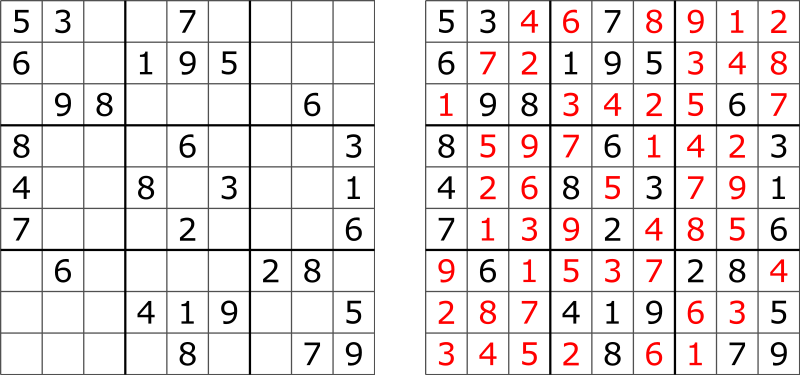
\includegraphics[width=0.8\textwidth]{img/sudokuexample}
			\caption{Left: Example of a sudoku puzzle with $n=m=3$. Right: The solved puzzle; original clues are in black, with the values to be entered shown in red.}\label{fig:example}
		\end{figure}
	\item
		Your code should be included in the appendix at the end of this file meant for that.
		The appendix should not be used for anything else.
\end{itemize}

\bibliography{report_template}

\clearpage
\appendix

\section*{Python files}
In this appendix, you must include all your Python files, so that the reviewers can evaluate your code.
So this must at least be your \texttt{sudokuai.py} file, but might include any support files.
Make sure that the file name (and path) is explicitly mentioned, so that it is clear how the code is used.
Avoid too-long code lines that need to be broken over multiple lines here.

\lstinputlisting[caption={Basic agent: \texttt{team00\_A2/sudokuai.py}}.]{sudokuai.py}

\lstinputlisting[caption={Agent with this: \texttt{team00\_A3/sudokuai.py}}.]{sudokuai.py}

\lstinputlisting[caption={Agent with that: \texttt{team00\_A3\_extra1/sudokuai.py}}.]{sudokuai.py}

\end{document}
